\documentclass{standalone}
\usepackage{tikz}
\usepackage{ctex,siunitx}
\setCJKmainfont{Noto Serif CJK SC}
\usepackage{tkz-euclide}
\usepackage{amsmath}
\usetikzlibrary{patterns, calc}
\usetikzlibrary {decorations.pathmorphing, decorations.pathreplacing, decorations.shapes,}
\begin{document}
\small
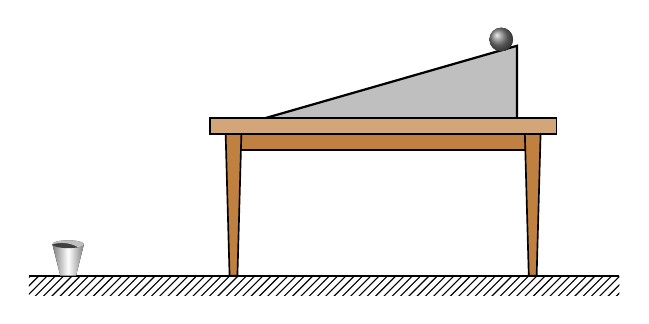
\begin{tikzpicture}[>=stealth,scale=1]
  \fill [pattern=north east lines](-4.5,-.25) rectangle (3,0);
  \draw [thick](-4.5,0)--(3,0);
  \draw [thick,fill=lightgray](-1.5,2) --(1.7,2.92)--(1.7,2);
  \draw [semithick,fill=brown!70](-2.2,1.8)rectangle(2.2,2);
  \draw [semithick,fill=brown](-1.9,1.8)rectangle(1.9,1.6);
  \draw [semithick,fill=brown](-2.0,1.8)--(-1.95,0)--(-1.85,0)--(-1.8,1.8)--cycle;
  \draw [semithick,fill=brown](2.0,1.8)--(1.95,0)--(1.85,0)--(1.8,1.8)--cycle;
  \fill [ball color=gray,semithick](1.5,3.0) circle (.15);
  \fill [left color=gray,right color=gray,middle color=white](-4.2,0.4)--(-3.8,0.4)--(-3.9,0)--(-4.1,0)--cycle;
  \fill [darkgray] (-4,0.4) ellipse(0.2 and 0.05);
  \fill [lightgray] (-4.2,0.4) arc( 180:-50:0.2 and 0.05)to[bend right=20]cycle;
\end{tikzpicture}
\end{document}